%File: formatting-instruction.tex
\documentclass[letterpaper]{article}
\usepackage{aaai}
\usepackage{times}
\usepackage{helvet}
\usepackage{courier}
\usepackage{url}
\usepackage{graphicx}
\frenchspacing
\pdfinfo{
/Title (Multi-Agent System Framework for Real-Time Strategy AI)
/Subject (AAAI Publications)
/Author (AAAI Press)}
\setcounter{secnumdepth}{0}  
 \begin{document}
% The file aaai.sty is the style file for AAAI Press 
% proceedings, working notes, and technical reports.
%
\title{Agent-Oriented Programming Framework Design for Real-Time Strategy AI}

\author{Antonio Arredondo\and Daniel Jaramillo\and Frank Navidad\and Ben Wright\\
New Mexico State University \\ Department of Computer Science \\ Box 30001 MSC CS \\ Las Cruces, NM 88003-8001
}

%%Blank authors for Double Blind Review
%\author{XXXXXX \and XXXXXXX \and XXXXXXX \and XXXXXXX \\
%123 Alphabet Lane \\  Somewheresville, NotYourState 11111-2222
%}

\maketitle
\begin{abstract}
\begin{quote}
In video game development, one of the many challenges for the developers is to create a challenging AI for the user.  Failure to create effective AI can cause the popularity of a game to decrease.  This can be particularly noticeable in Real-Time Strategy(RTS) games, where AI can either be too challenging or too predictable.  To address this problem, we present a Multi-Agent System Framework, KhasBot, to handle the Artificial Intelligence in a specific RTS Game, StarCraft: BroodWar.  By approaching the AI model as a subset of individual Agents capable of solving the common AI problems found in RTS games, for example, path-finding, resource allocation, task management and reactive planning.  This Framework will be tested in the SC AI 2011 competition.  In this paper we will discuss our reasoning for selecting JADE as our AI backbone, our design strategy, and our creation process in creating KhasBot.
%Results
\end{quote}
\end{abstract}

\section{Introduction}
Real-Time Strategy(RTS) Games are an area of interest in Artificial Intelligence(AI) Systems for many reasons.  They must adapt quickly to changing environments, make decisions on non-complete information, and involve multiple complex AI issues in general (for example, reactive planning, path-finding, and resource scheduling).  StarCraft, a RTS created by Blizzard in 1998, involves three different alien races in a battle for resources and superiority on a large variety of maps.  A human player of this game must keep track of many things at once, for example, resources, map locations, building placements and army units, including enemy player actions and locations.  The role of the player is to command their force of units and structures through mouse and keyboard; or in the case of our AI, the Broodwar API(BWAPI). Some players even operate at a level of 200-300 actions, or commands, per minute(APM) at very high levels of play. Our AI player will be designed to emulate high level players in the manner of unit control and strategy.

Controlling these units and structures throughout the game creates a dynamic and complex environment that poses a great challenge in creating an AI that can compete at expert levels.  For our AI, we selected one race to operate, the Protoss.  To get our AI functioning we will load it with pre-set build orders, a particular battle plan, and the means to execute those orders and plans.  Based on the enemy's race selection and map layout, our AI will proceed with one of the appropriate build orders.  As the game progresses, based on scouting information and enemy actions, we will change our build order accordingly in an effort to find the most effective way to defeat our opponent.  KhasBot, the name of our AI, at this stage, is being built for one-on-one battles.
%Outline Paragraph
For the remainder of the paper, we will discuss the some background of the BWAPI, JADE and RTS games, our design strategy and implementation, and finally our results.  We also mention some related and future work.

\section{Background}
What we do in this project is combine two different areas together, BWAPI  and Java Agent DEvelopment Framework(JADE).  StarCraft does not have any officially released AI API, so the BWAPI is injected into StarCraft at runtime, and through the used of a specially designed Proxy AI, the JADE Framework can interact externally with the game.  BWAPI and JADE are described in further detail below.

%Fill out
\subsection{Real-Time Strategy} %For Example in StarCraft
%What Real-Time is
Real-time strategy(RTS) games normally involve players commanding an army of units to build structures, collect resources and attack enemy players.
The player accomplishes this by issuing orders, normally through the keyboard and mouse on a computer, to individual or groups of units and structures.  By collecting needed resources on the map, the player can continue to build up their forces and bases.  For example, in StarCraft, the player would issue commands to a worker unit to collect minerals and vespene gas to be able to command another worker unit to build new structures or to order a building to create more units.  Through the use of effective map knowledge and time, the player can create a strategy that will lead to victory, which is usually defeating the enemy forces, capturing a target item or obtaining a certain resource goal.  For the StarCraft games our AI will be participating in, it will be focused on one-on-one matches with the goal of eliminating the enemy from the map.
%How the player does this
%Resource and unit management > node and map
%Strategy and Tactics
%Winning conditions


\subsection{BWAPI}
An issue with community development of AI for RTS games, and many games in general, is that many of them are closed source.  Users cannot directly program logic into the game and must use external tools to accomplish this.  For StarCraft, community members developed the BWAPI for directly injecting the logic into the game.  The BWAPI\footnote{\url{http://code.google.com/p/bwapi}} is an open-source Application Programming Interface (API) that enables AI creation for Starcraft: Broodwar.  It was developed in C++, but many extensions have allowed access to other languages such as Python, C\#, and Java.  For the purposes of KhasBot, Java has been used.

The BWAPI breaks down the StarCraft game into 5 basic objects: 
\begin{itemize}
\item \emph{Game}:  Holds all information about the current game being played, including known unit locations, resource nodes, etc. 
\item \emph{Player}:  Holds all information a player would have, for instance current resources, buildings, and controllable units.
\item \emph{Unit}: Represents a piece in the game, be it a mineral, building, or army unit.
\item \emph{Bullet}: Represents a projectile from an attack from units that are capable of ranged attacks.
\item \emph{Force}: Represents a collection of players attempting a singular objective.  This is similar to a co-operative description, where some players may be on the same team.
\end{itemize}

In addition to the game objects, a game control module \emph{AIModule.cpp} is injected as a \emph{dll} into the core StarCraft code.  This module contains the behaviours needed to process and execute commands in StarCraft.  This module can also use sockets to communicate outside of the game with other AI. For example, KhasBot is an external Java program running along with StarCraft, and our AI communicates through ProxyBot, which then relays our information to the AIModule.  An analogy to this can be that BWAPI is a tool-box, and the AIModule is a untrained worker on location with a radio, which is the ProxyBot.  Communicating through this radio is KhasBot, giving orders to the worker on how to operate the tools.

The basic flow of how BWAPI works is as follows, when the actual game begins BWAPI will call upon the \emph{onStart()} method from the \emph{AIModule} which will setup all the above objects with the begining of the game information.  After this, an \emph{onFrame()} method is called every frame of the game.  This is the looping method which holds all the reasoning and computational information of the actual AI.  The \emph{AIModule} returns orders to the StarCraft game via \emph{UnitCommand}s.  By giving Units in control of the AI player various actions or commands, (such as building, attacking, researching, and upgrading) the game can progress towards a conflict where either player can obtain victory. Victory is achieved when the AI player has eliminated the enemy force from the map.

\subsection{Agent-Oriented Programming}
Agent-Orient Programming is a Programming Paradigm started back in the 1990s.  The basis is to on the concept of 'agents' as opposed objects.  By doing this, one can focus more readily on the reasoning processes and communication paths of a system, rather than method calls\cite{AOP}.  Aside from communication, Agents can have a focused goal or set of goals to accomplish.

The basic flow of Agent-Oriented Programming, which our KhasBot is designed upon, is that Agents hold a set of beliefs and then based off changes (or additions) to them, the agents belief set will change, causing a possible reaction or change in the behaviour, or attempted actions, of said Agent.

For this particular framework, we used JADE (Java Agent DEvelopment Framework) to model our agents.  JADE is a Java middleware framework designed to handle and run agents developed from a package given by JADE.  JADE also handles running the agents platform along with all the communication\cite{JADEbook}.

%Must be added in for May 17th version
%\subsubsection{JADE}
%Agents, Behaviours, Platform and Messaging Protocols

\section{Related Work}
%Agent based papers, others, Overmind
We found that other researchers have approached this problem using other frameworks, some not explicitly agent based, to develop their AI.  A group of AI writers\cite{CrapPaper} used the BWSAL\footnote{\url{http://code.google.com/p/bwsal}} to implement a simple strategy with an agent minded outset.  We feel that, although they had modeled a sound agent system, they had a very limited test scope.

%McCoy Paper
A management design similar to ours (detailed later) build an agent framework for use in Open Source RTS\cite{McCoy}.  They implement their agent system using ABL in Wargus and have encouraging results.  They, however, only test their agent system against two scripted strategies and focus on different tasks than our own system.  

%BenWebers paper
Another implementation using ABL\cite{Weber} focused on reasoning to reactively change strategies.  They had positive results against the built-in AI, but less than positive against human players.  While they have a strong reasoning system, our system will be focused more on creating a modular framework.

%Overmind or other AI asides
Creators of the Overmind AI at UCBerkeley\footnote{\url{http://overmind.cs.berkeley.edu/}} created a successful StarCraft AI that uses reinforcement learning to individually control attack units with great precision.
At the time of this writing, we have not found any papers discussing the use of JADE in creating an AI for StarCraft: BroodWar.  More so, we have not found any using JADE for the development of AI Frameworks in video games.  This presents an opportunity for more future research.

\section{Design}
\subsection{Motivation}
In order to accomplish the task of creating an AI for StarCraft, we decided to approach by having each important task in the game represented by an Agent concerned with solving that task.  While an intuitive approach would be to represent each unit and structure as an agent, we quickly abandoned this due to many issues that design would entail such as coordination and cooperation of the units,  hardware allocation of that many threads at once, and actually being able to effectively communicate with BWAPI.

Instead, we conceptualized what the problem sets would potentially be and we came up with the following tasks: path-finding, resource management, placing buildings, controlling military units, and managing upgrades.  On top of these tasks, we also knew a few more agents would be needed to maintain and combine these problem sets to the goal of the current game.  Based on the idea that Agents are focused on one or two tasks, this lead to our current organization.   

\subsection{Organization}
% AI Motivation : Competing against high level players, knowledge of map, special properties, race match-ups, build orders of their opponent

Initially, our first design was based on the RTS AI framework, BWSAL.  However, this is developed in C++ and is not Agent-Based. The idea behind using an Agent-Oriented design was to offload reasoning of playing the RTS to individual agents that only focused on one facet of the overall problem.  We then split the problem into the following 7 agents(see Fig.\ref{fig:System}):
\begin{itemize}
\item \emph{Commander Agent} : Concerned with keeping the information up to date and controlling current active build orders.  The Commander Agent is the heart of KhasBot, it is also the communication gateway to and from StarCraft.  All game information passes through the Commander Agent and the Commander Agent processes all the commands to pass back to StarCraft.
\item \emph{Building Manager Agent} :  Concerned with placement of future buildings and builds structures based on the issued build order.  The building manager will analyze the current map data to determine where buildings can be placed and can communicate with the Unit Manager Agent to obtain a worker to build the planned building.
\item \emph{Structure Manager Agent} : Concerned with training units and upgrading technology.  Any command that would be normally issued by a player to a building is managed by this agent.
\item \emph{Battle Manager Agent} : Concerned with all combat matters including scouting, the act of sending a unit out into the fog-of-war to obtain valuable information.  The Battle Manager Agent controls all attack units, battle tactics, and makes decisions with those units based on scouting information, enemy movements and build orders.
\item \emph{Resource Manager Agent} : Concerned with all resource gathering, including "rate of" gathering, worker management and needed materials for segments of the build order.
\item \emph{Map Manager Agent} : Concerned with maintaining and updating map information and determines efficient path finding for any units in AI control.
\item \emph{Unit Manager Agent} : Concerned with maintaining unity between all the pieces used by the other Manager Agents and merging together unit commands for the Commander Agent.
\end{itemize}

In addition to the above agents, we also developed the \emph{Proxy Bot Agent}, that was in charge of interfacing with the BWAPI and getting the socket information from the StarCraft game and converting that information into messages the Agent System could understand.  It also converted messages from the Agent System to something the BWAPI and socket information understand.

\begin{figure}[hbp]
\begin{center}
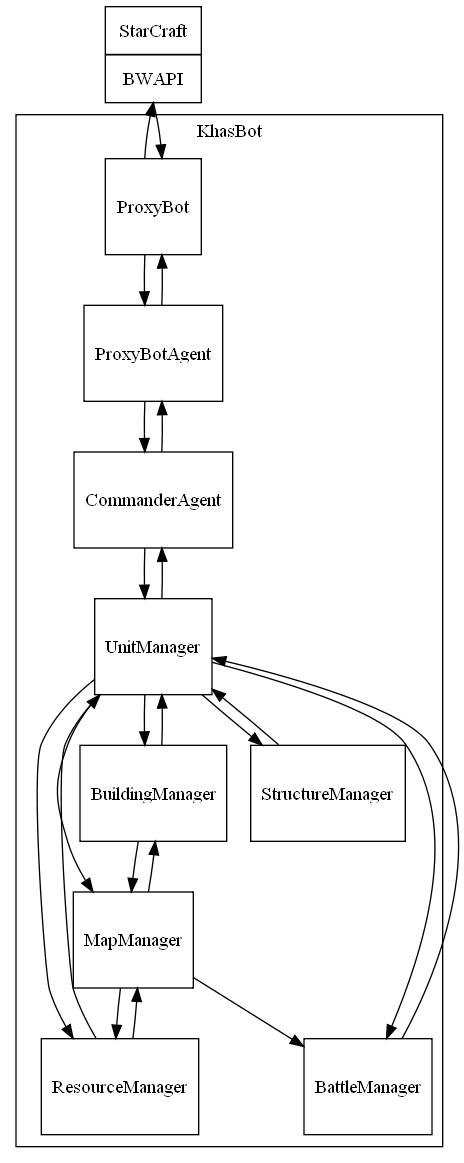
\includegraphics[scale=0.5]{TotalSystem.jpg}
\caption{Overall System Design for KhasBot}
\label{fig:System}
\end{center}
\end{figure}

Most of our Manager Agents follow a similar behavior to each other. Due to this, we were able to create a superclass KhasBotAgent that took care of most of the repetitive tasks.  With many agents working on separate areas, the key here is organizing their communication with each other.  Luckily, all of our protocols exhibit a request/inform type flow, which is a core design structure of the JADE Framework.  Game updates are sent to the \emph{Unit Manager Agent} by the \emph{Commander Agent} and all other managing agents are updated by the \emph{Unit Manager Agent} when relevant information changes to their goal.

The actual StarCraft Game is mapped to a \emph{GameObject} that the agents use to keep track of what they are doing.  As the game progresses, the Multi Agent System(MAS) continues to get game updates via a \emph{GameUpdateObject}, which is essentially a reduced game object.  The \emph{GameObject} is broken down into two different things, Player Information and Map Information. Map Information includes items like where is it safe to build or walk and what the starting locations are for the map in the game.  Player Information handles all units and ways the units can do research or upgrades.  These units include structures, mineral patches, and all other pieces in the game that can change.

\section{Implementation}
%TODO: Antonio should write some notes on this section and I'll edit it into the report, it would be great to have the agent figure
The basic idea that each Manager Agent follows is that they are each an agent inside of JADE that have multiple threaded behaviours that focus on different protocols between the various Manager Agents.

Due to the multiple behaviours at once, each agent heavily uses the DataStore ability from JADE, a central data location on the platform, to keep its information consistent with the other behaviours.

The main implementation of our Manager Agents can be found in our abstract class \emph{KhasBot Agent}. All other Manager Agents take this as a superclass. \emph{KhasBot} works on the following idea: all information for that Agent is stored in its own JADE DataStore, which is setup to be used by all behaviours of the agent. Since each agent has different behaviours, this is something that has to be overridden in their own \emph{setup()} method. All behaviours for the agents are \emph{ThreadedBehaviours} due to the fact that most of our behaviours are protocols between each Managing Agent and each protocol should not wait for a different protocol to finish, we found this to be the easiest way to implement non-preemption in JADE.

The communication, or protocols, of the Manager Agents falls into two categories, \emph{INFORM}'s or \emph{REQUEST}'s. We will discuss how \emph{Resource Manager Agent} is set up as an example:
% ANTONIO DOUBLE CHECK ME ON THESE NUMBERS
ResourceManagerAgent has up to 7 behaviours, 3 work as one-shot requests asking for either workers, minerals, or gas. The other 4 are longer lasting protocols that wait on updates of the game, respond to requests of worker needs or supply queries, and one last one to do the agents 'default' behaviour which is to assign workers to gather resources.

An important aspect of our Framework comes from the protocols between the agents and who can talk to who, \figure(Protocol-diagram} shows the links between all the managing agents.

%Agents and Default Behaviours

\subsection{Build Orders}
%Design related...
Build Orders are a part of StarCraft strategies that aim to follow a highly optimized, pre-set list of commands for the early part of a game.  These are used to provide a plan of attack to achieve victory.  One of the goals of our AI is to select or adjust the build-order on demand, based on map and scouting information.  In order to aid in lowering the complexity of our Agent Framework, we decided to implement an outside structure to maintain the list of commands the agents needed to complete.  This would allow us to apply different implementations and observe their effects on our AI.  The solution we choose to implement this was an external XML file.  This created an easy to manage medium that allows us to test different ideas within the structure without having to rebuild our framework.

The XML structure is based on the race selected and the in-game situation.  The strategy subsets are based on the supply resource and process the different commands held as sub-items when the required supply count is met.  The sub-items can be {\tt unit}, {\tt structure}, or {\tt action}.  The {\tt unit} item has attributes for the unit name.  The {\tt structure} item has attributes for the structure name and location of placement, which could be either a map location or near another structure.  The {\tt action} item has attributes for the action name, by name of the unit, location to achieve the action and importance.  For more advanced control in different in-game situations, it can maintain a list of commands for different opposing races and for each playable race.

The XML structure is loaded into an Java Object named \emph{BuildLoader} that will contain the list of orders. As the game progresses, the Commander Agent will send the current game information to \emph{BuildLoader}. It will look at the current in-game supply count and read specified list of commands for that condition. Updates for these commands are required before it will continue through the list.  An update will run through the list of commands up to the last supply count which it returned results to make sure everything is still true. These checks are made as the battle situation could change aspects of our build order. Special location constants will be asked from the Unit Manager Agent which will allow \emph{BuildLoader} to check the location of a new structure that will be created in-game and determine if they are close to where a certain structure needs to be built. Unit item commands will notify the Commander Agent to tell the Unit Manager Agent that specified unit needs to be created. Action commands will work the same way by providing an action for a named unit type, for example, scout action to a probe or attack to a group of battle units.

\section{Results}
%TODO: This will change as more things are added to KhasBot
%Refer to other agent paper
%APM, Win/Loss, Overall Performance
Initial tests have been positive.  The message passing between agents have resulted in simple build orders being executed.

\section{Conclusion and Future Work}
We have found that building StarCraft AI is viable using an Agent-Oriented Programming Framework.  The communication structure established by JADE allowed us to create agents capable of specific goals and relaying information based on those goals to other agents and to StarCraft
%Evaluate after paper is close to complete.
[[this sentence is remarkably vague while sounding not]].  Splitting the computation needed in an AI among agents provides another avenue for creating StarCraft AI and ultimately video-game, military, or management AI.

In the future, we will continue to refine KhasBot with more build orders and potential decisions for those build orders.  We will also look into generalizing KhasBot for all three races, as our Build Order parser will allow for that.

\bibliography{bibliography}{}
\bibliographystyle{aaai}

\end{document}
